\documentclass{article}
\usepackage{graphicx} % Required for inserting images
\usepackage{tabularx}
\usepackage{amssymb}
\usepackage{amsmath}
\usepackage{amsthm}
\usepackage{listings}
\usepackage[swedish]{babel}
\usepackage{hyperref} 
\usepackage{mathtools}
\usepackage{color}
\usepackage{titlesec}
\usepackage{sectsty}
\usepackage[a4paper, margin=2cm]{geometry}
\usepackage{booktabs}
\usepackage{caption}
\usepackage{subcaption}
\usepackage{float}


\renewcommand{\thesection}{\arabic{section}.}
\renewcommand{\thesubsection}{\alph{subsection})}
\subsectionfont{\normalfont\bfseries\fontsize{10}{12}\selectfont}

\title{SF1930 Projekt}
\author{Vilhelm Karlin}
\date{\today}

\begin{document}
\maketitle

\section{Uppvärmning}
\subsection{Alla betyg i dataramen är för närvarande tal mellan 0 och 10. 
Normalisera dessa värden i dataramen så att de är mellan 0 och 1.}

För att normalisera datan så itererade jag helt enkelt över de relevanta kolumnerna och dividerade varje värde med 10. 

\subsection{Gör ett histogram för alla trickbetyg för trick 1-4. Vad observerar du? 
Finns det ett visst värde som dyker upp oftare än de andra? Om så är fallet, hur står detta värde i jämförelse med de andra?}

Som syns i figur Fig\ref{fig:1b} så är det enskilt vanligaste värdet 0. Resterande värden är ungefär grupperande mellan 0.7 och 0.9.
Inga värden finns mellan 0.1 och 0.4.

\subsection{For varje trick 1-4 skapa en ny kolumn med namnet 'make i' för i = 1, 2, 3, 4 så att värdet av 'make i' i en given rad är 1 om skateboardåkaren landade trick i och 0 annars.}
Detta implementeras enkelt genom att introducera fyra nya kolumner, en för varje trick. Dessa fylls sedan med 1 om skateboardåkaren landade trick i och 0 annars.

\subsection{För varje skateboardåkare skatta sannolikheten att ett trick får ett betyg som är större än 0.6 givet att 
skateboardåkaren landar tricket. Vad är sannolikheten att skateboardåkaren inte lyckas landa ett visst trick? Vad observerar du? 
Relatera dina observationer till era observationer i del (b).}

Som syns i Tab\ref{tab:1d} så är det endast två skateboardåkare som inte fick betyg större än 0.6 på något av sina gjorda trick.
Detta rimmar väl med observationerna i Fig\ref{fig:1b} där värdena antingen var 0 eller större än runt 0.6.

\subsection{Gör ett spridningsdiagram för runbetyg 1 mot runbetyg 2. Ser du någon tydligt korrelation från diagrammet?}

Korrelationen mellan runbetyg 1 och runbetyg 2 är väldigt svag och ingen tydlig trend kan urskiljas i Fig\ref{fig:1e}.
Korrelationskoefficienten $\rho = 0.19$, vi kan därmed betrakta run 1 och run 2 som oberoende av varandra.

\clearpage  % Start a new page for figures and tables

\begin{figure}[htbp]
    \centering
    
    \begin{minipage}{0.45\textwidth}
        \centering
        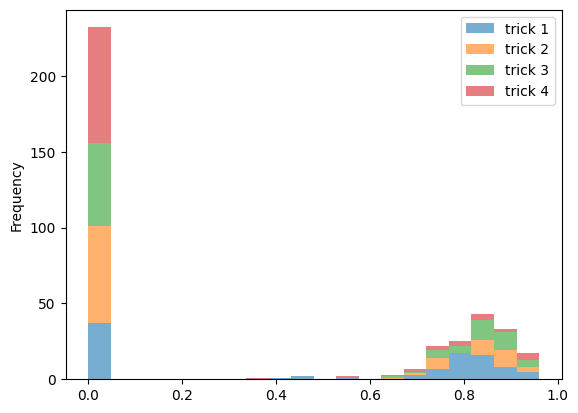
\includegraphics[width=\textwidth]{Figures/1b.png}
        \caption{Histogram för trickbetyg 1-4.}
        \label{fig:1b}
    \end{minipage}
    \hfill
    \begin{minipage}{0.45\textwidth}
        \centering
        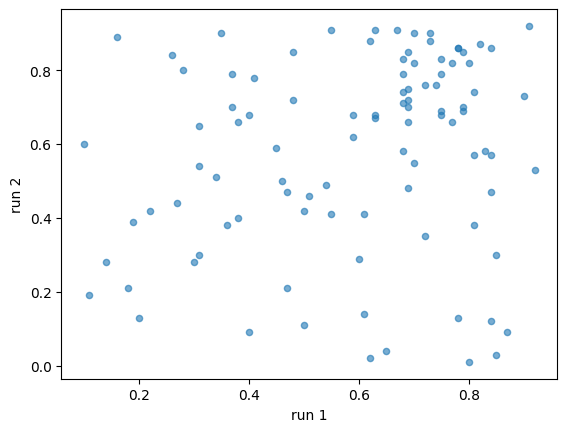
\includegraphics[width=\textwidth]{Figures/1e.png}
        \caption{Caption for figure 2.}
        \label{fig:1e}
    \end{minipage}
    
\end{figure}

\begin{table}[htbp]
    \centering
    \begin{tabular}{lrr}
      \toprule
      \textbf{ID} & \textbf{Gjorda trick} & \textbf{Andel med betyg större än 0.6} \\
      \midrule
      Berger     &      2 &              1.00 \\
      Decenzo    &      7 &              1.00 \\
      Eaton      &      5 &              1.00 \\
      Foy        &      6 &              1.00 \\
      Fynn       &      6 &              1.00 \\
      Gustavo    &      8 &              1.00 \\
      Hoban      &      8 &              1.00 \\
      Hoefler    &      7 &              1.00 \\
      Horigome   &      9 &              1.00 \\
      Huston     &      3 &              1.00 \\
      Jordan     &      8 &              1.00 \\
      Joslin     &      9 &              1.00 \\
      Majerus    &      3 &              0.33 \\
      McClung    &      1 &              0.00 \\
      Midler     &      4 &              1.00 \\
      Milou      &      9 &              1.00 \\
      Mota       &      3 &              1.00 \\
      Oliveira   &      5 &              1.00 \\
      O’neill    &      3 &              1.00 \\
      Papa       &      7 &              1.00 \\
      Pudwill    &      3 &              0.33 \\
      Ribeiro C  &      3 &              1.00 \\
      \bottomrule
    \end{tabular}
    \caption{Betyg större än 0.6 givet att skateboardåkaren landar tricket}
    \label{tab:1d}
\end{table}
\newpage

\section{En frekventistisk modell.}
\subsection{Ge en punktskattning för varje \texorpdfstring{$\theta_i$}, sannolikheten att skateboardåkaren i landar ett trick.}


\end{document}